\documentclass[10pt]{beamer}

\usefonttheme[onlymath]{serif}
\usetheme[progressbar=frametitle]{metropolis}
\usepackage{appendixnumberbeamer}
\usepackage{notation}

\usepackage{booktabs}
\usepackage[scale=2]{ccicons}

\usepackage{pgfplots}
\usepgfplotslibrary{dateplot}

\usepackage{xspace}
\newcommand{\themename}{\textbf{\textsc{metropolis}}\xspace}

\bibliographystyle{unsrtnat}

\title{Συναρτησιακή γλώσσα για χρήση στο blockchain}
\subtitle{Μεταγλώττιση αμοιβαία αναδρομικών τύπων}
% \date{\today}
\date{}
\author{Γκούμας Βασίλης}
\institute{Εθνικό Μετσόβιο Πολυτεχνείο}

\vspace{1cm}

\titlegraphic{\hfill
\includegraphics[height=2cm]{images/pyrforos.pdf}}


\begin{document}

\maketitle

\begin{frame}{Περιεχόμενα}
  \tableofcontents[hideallsubsections]
\end{frame}

\section{Εισαγωγή}


\begin{frame}[fragile]{Εισαγωγή}

  Η παρούσα διπλωματική εκπονήθηκε σε συνεργασία με την ομάδα
  γλωσσών της IOHK
 \begin{center}
    
\includegraphics[width=1cm,height=0.8cm,keepaspectratio]{images/iohk-symbol.png}
  \end{center}

\end{frame}


\begin{frame}[fragile]{Ενδιάμεσες αναπαραστάσεις}
 Οι μεταγλωττιστές και οι εικονικές μηχανές (VMs) κάνουν συχνά έντονη χρήση
 των ενδιάμεσων αναπαραστάσεων κατά την μεταγλώττιση.

 \begin{itemize}
    \item  απλότητα + εκφραστικότητα
    \item  διευκολύνει τα επόμενα περάσματα
    \item  δημιουργία API μεταξύ μεταγλωττιστών
  \end{itemize}

\end{frame}

\begin{frame}{Παραδείγματα}

\begin{columns}[T,onlytextwidth]
    \column{0.4 \textwidth}
      Χαμηλού επιπέδου
      \begin{itemize}
        \item Java Bytecode
        \item RTL
        \item LLVM IR
      \end{itemize}

    \column{0.4 \textwidth}
      Υψηλού επιπέδου
      \begin{itemize}
          \item  GHC Core
        \item Idris TT
       \item Ocaml Lambda
      \end{itemize}
\end{columns}

\end{frame}



\begin{frame}{Συναρτησιακές IR}

Βασισμένες συνήθως σε παραλλαγές του λ-λογισμού.

    \begin{alertblock}{Μειονεκτήματα}
	\begin{itemize}[]
	    \item Δύσκολο να γραφτούν και να διαβαστούν
	    \item Κάνουν μεγάλο το βήμα της μεταγλώττισης από μία γλώσσα υψηλού επιπέδου στον λ-λογισμό.
	    \item Πιο δύσκολες για κάποιες βελτιστοποιήσεις
	\end{itemize}
	\end{alertblock}
\end{frame}

{
\setbeamercolor{background canvas}{bg=white}
\begin{frame}{GHC}
%\begin{columns}
\begin{columns}[T,onlytextwidth]
\column{0.33 \textwidth}
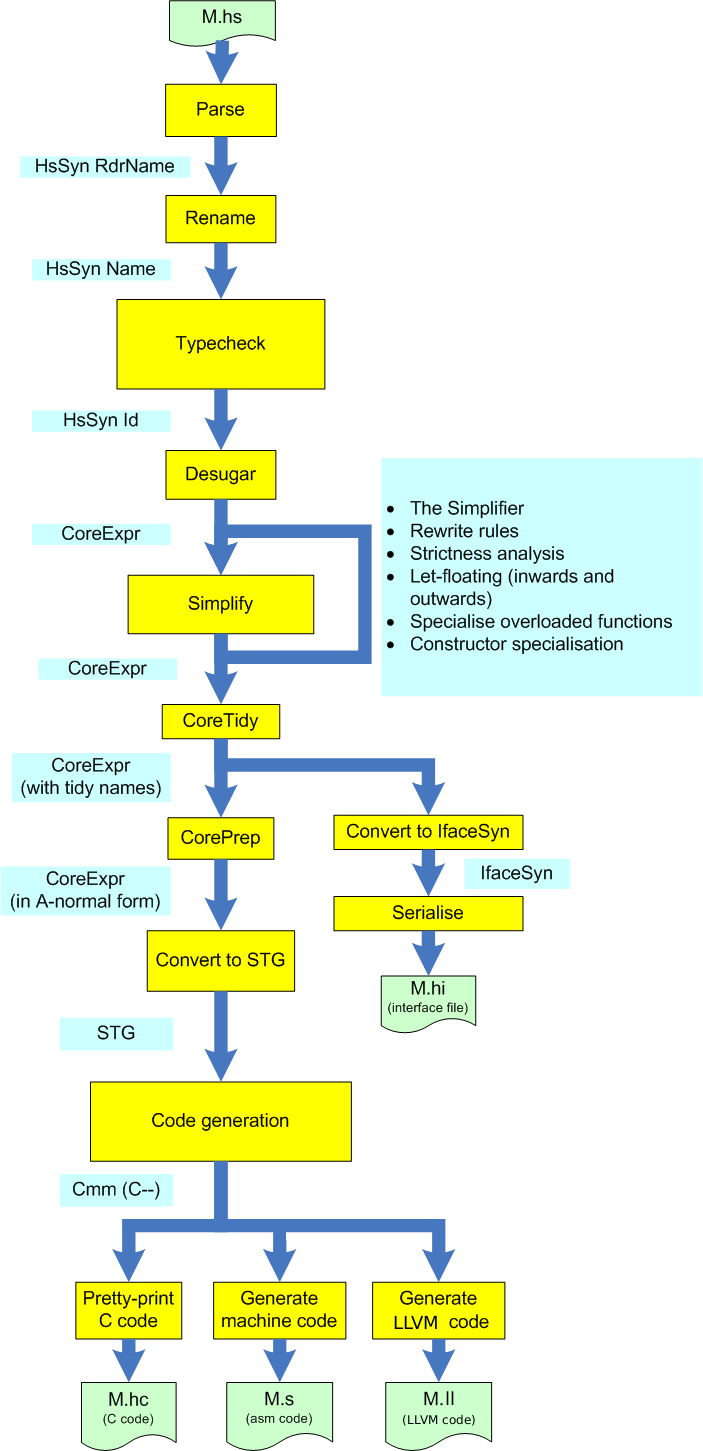
\includegraphics[scale=0.15]{images/ghc.png}

\column{0.60 \textwidth}
      O GHC χρησιμοποιεί \textbf{3} ενδιάμεσες αναπαραστάσεις κατά
      την μεταγλώττιση από κώδικα Haskell σε κώδικα μηχανής
\\
(και πολλά περάσματα)
      \begin{itemize}
        \item GHC Core
        \item STG
        \item Cmm
      \end{itemize}
  \end{columns}
\end{frame}
}

\section{Blockchain}

\begin{frame}[fragile]{Bitcoin}

Η τεχνολογία του blockchain εισήχθηκε πρώτη φορά το 2008, από τον Satoshi Nakamoto.

Το bitcoin είναι το πρώτο ψηφιακό νόμισμα που λύνει το πρόβλημα του double
spending.
Μπορούμε να αποφασίσουμε ποιος έχει τι χωρίς την μεσολάβηση κεντρικής αρχής

\end{frame}

\begin{frame}[fragile]{Smart contracts - Τότε}

    Η ιδέα των \textit{έξυπνων συμβολαίων} (smart contracts), προηγείται του Bitcoin.
    \begin{itemize}
        \item συζητήθηκε για πρώτη φορά από τον Nick Szabo, το 1994
        \item η ιδέα στοχεύει στον συνδυασμό του software/hardware με
        συμβόλαια \textbf{νομικού} χαρακτήρα
        \item αυτόματη εκτέλεση συμβολαίων με λιγότερα κόστη
    \end{itemize}

\end{frame}

\begin{frame}[fragile]{Smart contracts - Τώρα}

    Πλέον με τον όρο smart contract αναφερόμαστε σε οποιονδήποτε
    υπολογισμό γενικής φύσεως που εκτελείται πάνω από κάποιο blockchain



\begin{alertblock}{Πλεονεκτήματα}
    \begin{itemize}
        \item Self-verifiable
        \item  Self-executable
        \item Tamper Proof
        \item \alert{απαλοιφή μεσάζοντα}
    \end{itemize}
\end{alertblock}

\end{frame}


%\begin{frame}[fragile]{Smart Contracts - Ethereum}

%Το Ethereum \citep*{wood2014ethereum} ήταν το πρώτο ψηφιακό νόμισμα που χρησιμοποίησε
%Turing-Complete γλώσσα για τον προγραμματισμό συμβολαίων
%\end{frame}

\begin{frame}{Smart Contracts - Παραδείγματα Εφαρμογών}

\begin{itemize}
    \item DAO (Decentralized Autonomous Organizations)
    \item μεταφορά ιδιοκτησίας
    \item εκκαθάριση πληρωμών
\end{itemize}

\end{frame}

\begin{frame}{Smart Contract hacks}

\begin{description}[leftmargin=-.5in]
\item<1->[ ~~~~~~~DAO hack] (2016) 3.6m Ether, 15\% του συνολικού όγκου σε κυκλοφορία
\item<2->[Parity wallet hack] (Ιούλιος 17) 150.000 Ether
\item<3->[Parity Freeze hack] (Νοέμβριος 2017) 513.774 Ether
\end{description}

\only<4>{
Τα παραπάνω hacks οφείλονται σε λάθη κατά την υλοποίηση
των smart contracts που ελέγχουν τα tokens.
}

\end{frame}

\begin{frame}{Γλώσσες για smart contracts}

\begin{itemize}

\item<1-> Η χρήση γλωσσών όπως η Solidity (βασισμένη στην javascript)
αποτελεί εμπόδιο για τυπική ανάλυση των συμβολαίων.

\item<2-> Χρειαζόμαστε  τυπικές μεθόδους ανάπτυξης και έλεγχου των
έξυπων συμβολαίων, όταν οι αποτυχίες κοστίζουν ακριβά, χωρίς μια κεντρική αρχή να διορθώσει την ζημιά.
\item<3->
Η ανάγκη για σφάλεια στα έξυπνα συμβόλαια και ο έλεγχος ότι κάνουν μόνο αυτό που πρέπει να κάνουν καθιστά την χρήση σωστών πρακτικών ανάπτυξης και την επιστράτευση των formal methods αναγκαιότητα.
\item<4->
Η χρήση συναρτησιακής γλώσσας προλαβαίνει αρκετά bugs και διευκολύνει
την χρήση πιο χρονοβόρων μεθόδων.
\end{itemize}

\end{frame}


\begin{frame}{Γλώσσες για smart contracts}
Το σύστημα τύπων και η ευκολία ανάλυσης κάνει τις
συναρτησιακές γλώσσες την κατάλληλη επιλογή για πραγματικές πλατφόρμες έξυπων συμβολαίων
\begin{itemize}
    \item
    Simplicity - blockstream
    \item
    Michelson - tezos
    \item
    Plutus - iohk
    \end{itemize}


\end{frame}

\begin{frame}{Plutus}
Αρχιτεκτονική προγραμματισμού έξυπων συμβολαίων σε Haskell ,
κάνει χρήση τεχνικών staged metaprogramming

    \begin{itemize}
        \item Ένα GHC plugin αναλαμβάνει την μεταγλώττιση του κώδικα Haskell
        \item Ο χρήστης γράφει μαζί τον on-chain κώδικα που
        θα ανέβει στο blockchain, με τον off-chain βοηθητικό κώδικα
        \item On και off chain κώδικας μεταγλωττιζόνται ξεχωριστά
        \begin{itemize}
            \item  O οn-chain κώδικας μεταγλωττίζεται σε \FIR{} και στη συνέχεια
            σε Plutus Core
            \item  Ο off-chain κώδικας μεταγλωττίζεται ως έχει σαν κώδικας
            Haskell
        \end{itemize}

     \end{itemize}
\end{frame}

\section{ System F}

\begin{frame}{\FOM}

\begin{itemize}
    \item Προσθέτει πολυμορφισμό στον  απλό λ-λογισμό
    \item Υποστηρίζει συναρτήσεις στο επίπεδο των τύπων (όχι ιδιαίτερα χρήσιμες από μόνες τους) κάνοντας δυνατή την έκφραση τύπων δεδομένων στο επίπεδο της γλώσσας
    \item Γίνεται computation στο επίπεδο των τύπων (strongly normalizing)
    \item \alert{Χρειαζόμαστε την αναδρομή!}
    \end{itemize}

\end{frame}

\begin{frame}{Αναδρομικοί τύποι}
    \begin{itemize}
    \item
    Οι αναδρομικοί τύποι μπορούν να εκφραστούν ως fixpoint συναρτήσεων
    τύπων.ου
    \item[]<1->
    \begin{displaymath}
         \textbf{List} ~a = \textbf{Nil} ~|  ~\textbf{Cons} ~a  ~(\textbf{List} ~a)
        \end{displaymath}
    \item[]<2->
    Ένας τύπος θεωρείται ισομορφικός με το ξετυλιγμά του
    \item[]<3->
         $\List = \mu \alpha. \tau = \mu \alpha. 1 + \alpha*\List$ \\
    \item[]<4->
        % $\mu X . int + int * X  = \mu X. \tau $
         $\unwrap (\mu \alpha. \tau) = \tau\{\mu \alpha. \tau / \alpha\} =
         1 + \alpha * (\mu \alpha. \tau)$ \\
    \item[]<5->
        $ \wrap ( 1 + \alpha * (\mu \alpha. \tau)) =
         \mu \alpha. \tau$ \\
    \end{itemize}
\end{frame}

\begin{frame}{Αναδρομικοί Τύποι}

\begin{itemize}
\item[]
\begin{align*}
 \texttt{fix} \ f &= f \ (\texttt{fix} \ f)   \\
\textbf{List} ~a &= \texttt{fix} (\lambda r . \Lambda a. 1 + a * r) \\
&= (\lambda r. \Lambda a. 1 + a * r) (\texttt{fix} \ \lambda r. \Lambda a. 1 + a * r)  \\
&= \Lambda \alpha. 1 + a*(\texttt{fix} \lambda r. \Lambda a. 1 + a * r)) \\
 &= \Lambda a. 1 + a * \textbf{List} ~a \\
 &= \cdots \\
&= \Lambda \alpha. 1+ a * \cdots * a \\ 
\end{align*}

 \item<2-> παραλλαγή στον fixpoint operator:

        $\ifix :: ((k -> *) -> (k -> *)) -> (k -> *)$
        αντί για τον κλασσικό \\
        $\texttt{fix} :: (k -> k) -> k$
    \end{itemize}

\end{frame}


\setbeamercolor{background canvas}{bg=white}
\begin{frame}{Γραμματική της \FOMF}
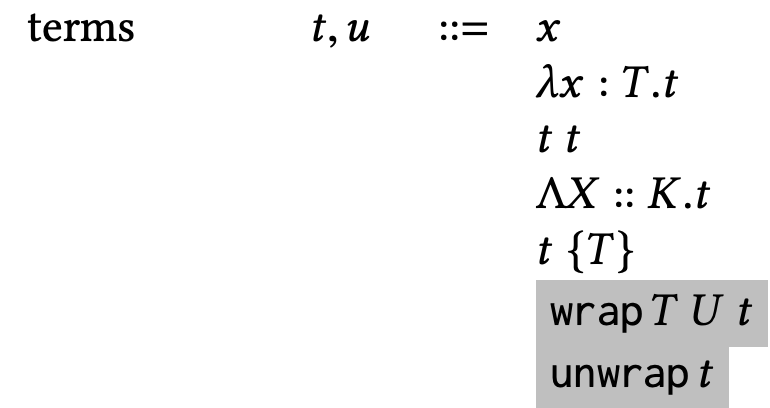
\includegraphics[scale=0.5]{images/terms.png}
\end{frame}

\begin{frame}{Τύποι στην \FOMF}
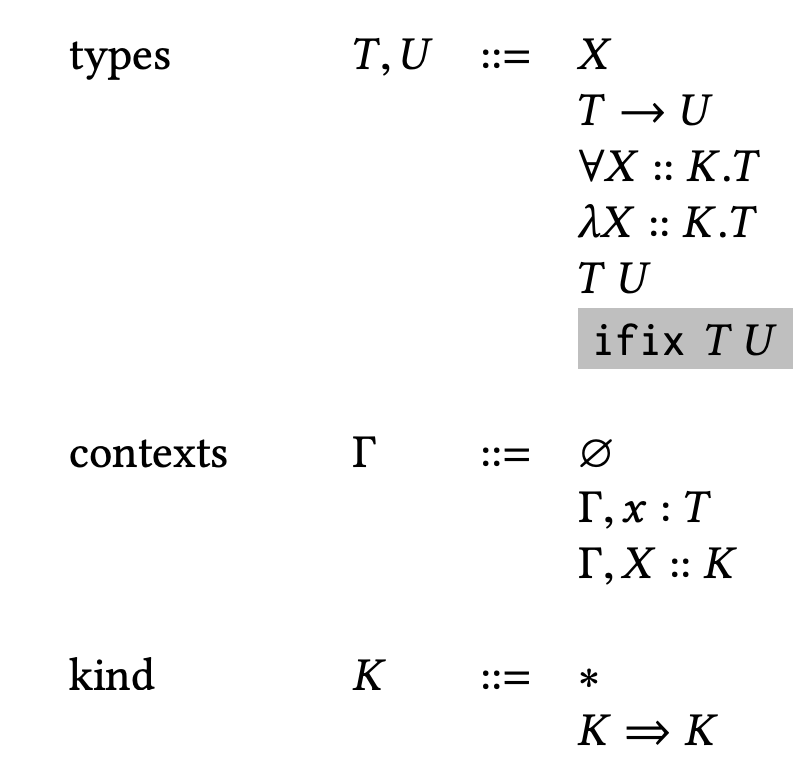
\includegraphics[scale=0.5]{images/types.png}
\end{frame}


\begin{frame}{\FOM}

    \begin{itemize}[<+->]
    \item[] {\inference[T-Var]{x:T \in \Gamma}{\Gamma |- x:T}}

    \item[]
    \inference[T-Abs]{\Gamma, x:T_1 |- t:T_2 & \Gamma |- T_1 :: \Type}{\Gamma |- (\lambda x:T_1.t) : T_1 -> T_2}

    \item[]
    \inference[T-App]{\Gamma |- t_1 : T_1 -> T_2 & \Gamma |- t_2 : T_1}{\Gamma |- (t_1 ~ t_2) : T_2}

    \item[]
    \inference[T-TAbs]{\Gamma, X::K |- t:T }{\Gamma |- (\Lambda X::K.t) : (\forall X::K.T)}

   \item[]
   \inference[T-TApp]{\Gamma |- t_1: \forall X::K_2.T_1  & \Gamma |- T_2 :: K_2}{\Gamma |- (t_1 ~\{T_2\}) : \subst{X}{T_2}{T_1}}
    \end{itemize}

\end{frame}

\begin{frame}{Σύστημα Τύπων της \FOMF}

 \begin{displaymath}
    \begin{array}{ll}
   \multicolumn{2}{l}{\inference[T-Wrap]{\Gamma |- M: (F ~( \lambda (X :: K). \ifix F ~X)) ~T & \Gamma |- T:: K \\ \Gamma |- F :: (K\kindArrow\Type)\kindArrow (K\kindArrow\Type)}
            {\Gamma |- \wrap ~ F ~ T ~ M : \ifix F ~T}  }\\
    \\ \\ \\ 
    \multicolumn{2}{l}{\inference[T-Unwrap]{\Gamma |- M : \ifix F ~T & \Gamma |- T :: K }
            {\Gamma |- \unwrap M : (F ~( \lambda (X :: K). \ifix F ~X)) ~T  }  }\\
    \\
     \end{array}
    \end{displaymath}
\end{frame}

\begin{frame}{\FOMF}


\FOMF ~= ~\FOM + αναδρομικοί τύποι

\FIR ~= ~\FOMF ~+ \texttt{let} bindings

\end{frame}

\begin{frame}{\FIR{}}
Θα ορίσουμε την ενδιάμεση γλώσσα \FIR{}, η οποία επεκτείνει     την    \FOMF
       ~ με τα  εξής χαρακτηριστικά:
    \begin{itemize}
        \item <2->Όρους \texttt{let} μη αναδρομικών όρων, τύπων και τύπων δεδομένων
        \item <3-> Όρους \texttt{let} αναδρομικών τύπων και τύπων δεδομένων
    \end{itemize}


\end{frame}


\begin{frame}{\FIR{}}
Θα ορίσουμε την ενδιάμεση γλώσσα \FIR{}, η οποία επεκτείνει την \FOMF
~ με τα εξής χαρακτηριστικά:
    \begin{itemize}
        \item Όρους \texttt{let} μη αναδρομικών όρων, τύπων και
         \alert{τύπων δεδομένων}
        \item Όρους \texttt{let} \alert{αναδρομικών} τύπων και
        \alert{τύπων δεδομένων}

    \end{itemize}
    Εμείς θα εστιάσουμε στους τύπους δεδομένων (datatypes)
\end{frame}
\setbeamercolor{background canvas}{bg=white}


%\begin{frame}{Αλγεβρικοί Τύποι δεδομένων}
%Οι συναρτησιακές γλώσσες υποστηρίζουν \textit{αλγεβρικούς τύπους δεδομένων}
%(Algebraic Data Types)
%  \metroset{block=fill}
% \begin{exampleblock}{Παράδειγμα}
%     Maybe a = Nothing | Just a    \\
%     List a = Nil | Cons a (List a)
%\end{exampleblock}
%\end{itemize}
%\end{frame}

\begin{frame}{Συμβολισμός}

Στα παρακάτω, με
$\seq{a}$
θα συμβολίζουμε την ακολουθία
$ a_1, \ldots, a_n$

\end{frame}


\begin{frame}{\texttt{Let}-bindings στην \FIR{} }

\begin{itemize}
    \item <1->Η \FIR{} υποστηρίζει την δήλωση (αναδρομικών) όρων και ADTs με την χρήση
\texttt{let}-binding.
    \item <2->Η μόνη επέκταση που γίνεται στην \FOMF ~είναι:

\item[]<3->{
%\begin{itemize}
  \begin{displaymath}
  \begin{array}{lllll}
                  &   & \tlet ~ [\rec] ~ \seq{b} ~ \tin ~ t & &\\
                      &        &     &                             &   \\
     b      & ::= & x : T = t     &   & \\
                              &     & X :: K = T      & &\\
                            &     & \datatype{X}{(\seq{Y :: K})}{x}{\seq{c}} &   &\\
 \end{array}
  \end{displaymath}
 %\end{itemize}
}
\item[] \only<4>{$$
\datatype{\Maybe}{(A :: \Type)}{\textsf{matchMaybe}}{(\Nothing (), \Just (A))}$$
}
\end{itemize}

\end{frame}



\begin{frame}[fragile]{Μη αναδρομικά \texttt{let}-bindings }

Η μεταγλώττιση των \texttt{let}-όρων για μη αναδρομικούς όρους και τύπους
είναι απλή:

\begin{displaymath}
    \begin{array}{lll}
    \compileterm(\tlet x : T = b \tin v) &=& (\lambda (x : T) . v)\ b\\
    \\
    \end{array}
\end{displaymath}

\end{frame}



\begin{frame}[fragile]{Μη αναδρομικά \texttt{let}-bindings }

Η μεταγλώττιση των \texttt{let}-όρων για μη αναδρομικούς όρους και τύπους
είναι απλή:

\begin{displaymath}
    \begin{array}{lll}
    \compileterm(\tlet x : t = b \tin v) &=& (\lambda (x : t) . v)\ b\\
    \\
    \compiletype(\tlet X :: K = b \tin v) &=& (\Lambda (X :: K) . v)\ \{b\}
    \end{array}
\end{displaymath}

\end{frame}

\begin{frame}{Κωδικοποίηση Scott}
Στην κωδικοποίηση Scott, ένας αλγεβρικός τύπος δεδομένων ταυτίζεται με την
συνάρτηση που τον καταστρέφει

\begin{itemize}
    \item[]
\begin{displaymath}
 Bool = \forall R . R \rightarrow R \rightarrow R
\end{displaymath}
\item[]
\begin{displaymath}
 SNat =  \forall R . R \rightarrow (SNat \rightarrow R) \rightarrow R
\end{displaymath}

\item[]
\begin{displaymath}
 List = \lambda (a :: *) ->
  \forall (r :: *) . r -> (a -> List ~ a -> r) -> r
\end{displaymath}

\end{itemize}

\end{frame}

\begin{frame}{Κωδικοποίηση Scott}
\begin{itemize}
\item[]
    \begin{displaymath}
    Maybe = \lambda(a :: *) ->
  \forall (r :: *) . (a -> r) -> r -> r
    \end{displaymath}

\item[]
\begin{displaymath}
Just = \Lambda(a :: *) -> \lambda(arg : a) ->
  \Lambda(r :: *) ->  \\
    \lambda (branch_{Just} :: a -> r)
     (branch_{Nothing} :: r) ->
        branch_{Just} ~arg
\end{displaymath}

\end{itemize}

Οι κατασκευαστές επιλέγουν το κατάλληλο branch \\
\alert{Το pattern matching είναι η εφαρμογή συναρτήσεων}

\end{frame}


\begin{frame}{Αμοιβαία αναδρομικοί τύποι δεδομένων}

Αμοιβαία αναδρομικοί ADTs , βρίσκουν
  \begin{itemize}[<+- | alert@+>]

    \item ορισμό γραμματικών για γλώσσες
    \item αναπαράσταση δέντρων σύνταξης (AST)
    \item
   Ιδιαίτερα χρήσιμο χαρακτηριστικό για γλώσσα που προορίζεται
    για συγγραφείς μεταγλωττιστών
\end{itemize}


\end{frame}

\section{Μεταγλώττιση αναδρομικών ADTs}

\begin{frame}{Μεταγλώττιση αναδρομικών τύπων}
 \begin{displaymath}
      \begin{array}{l@{\ }l@{\ }l}
 \multicolumn{3}{l}{\textsf{Στις παρακάτω διαφάνειες έχουμε:}}\\
  \multicolumn{3}{l}{l = \tlet \rec \seq{d} \tin t} \\
  \multicolumn{3}{l}{d = \datatype{X}{(\seq{Y :: K})}{x}{(\seq{c})}} \\
  \multicolumn{3}{l}{c = x(\seq{T})}\\
  \\
    \end{array}
    \end{displaymath}


\end{frame}

\begin{frame}{Μεταγλώττιση αναδρομικων τύπων}
Το τέχνασμα είναι η χρήση tags για κάθε στοιχείο της αμοιβαία αναδρομικής
οικογένειας , στο επίπεδο των τύπων. Αφού έχουμε την κατάλληλη μορφή
μπορούμε να εφαρμόσουμε τον τελεστή ifix.

Η εκφραστικότητα της \FOMF ~επιτρέπει συναρτήσεις στο επίπεδο των τύπων,
γεγονός που μας επιτρέπει να εκφράσουμε παραμετροποιημένους τύπους


\end{frame}


\begin{frame}{Μεταγλώττιση TreeForest}

\begin{align*}
d_1 &\defeq \datatype{\Tree}{A}{\textsf{matchTree}}{(\Node (A, \Forest A))}\\
d_2 &\defeq \datatype{\Forest}{A}{\textsf{matchForest}}{(\NNil(), \CCons(\Tree A, \Forest A))}
\end{align*}

\end{frame}

\begin{frame}{Μεταγλώττιση TreeForest}

\begin{itemize}[<+->]
  \item $\tagKind{l}$ εκφράζει το kind των datatypes της οικογένειας,
  με κωδικοποίηση Scott του γινομένου (tuple)
    $$\tagKind{l} = (\Type \kindArrow \Type) \kindArrow (\Type \kindArrow \Type) \kindArrow \Type$$
  \item $\dtTag{l}{d}$ το tag για κάθε datatype της οικογένειας
    \begin{align*}
    \dtTag{l}{\Tree} &= \lambda A . \lambda (v_1 :: \Type \kindArrow \Type) (v_2 :: \Type \kindArrow \Type) . v_1\ A\\
    \dtTag{l}{\Forest} &= \lambda A . \lambda (v_1 :: \Type \kindArrow \Type) (v_2 :: \Type \kindArrow \Type) . v_2\ A
    \end{align*}
  \item $\dtInst{f}{l}{d}$ αρχικοποιεί την οικογένεια $f$ του
    datatype $d$ εφαρμόζωντάς το αντίστοιχο tag.
    \begin{align*}
    \dtInst{f}{l}{\Tree} &= \lambda A . f\ (\dtTag{\seq{d}}{\Tree}\ A)\\
    \dtInst{f}{l}{\Forest} &= \lambda A . f\ (\dtTag{\seq{d}}{\Forest}\ A)
    \end{align*}
\end{itemize}
\end{frame}

\begin{frame}{Μεταγλώττιση TreeForest}

\begin{itemize}
 \item $\dtFamily{l}$ ο τύπος της αμοιβαία αναδρομικής οικογένειας τύπων
 Παίρνει το αναδρομικό όρισμα και το tag και αρχικοποιεί τους τύπους με το
 αναδρομικό όρισμα.
    \begin{align*}
    \dtFamily{l} =&\ \lambda r\ t . \tlet \\
        &\quad\Tree = \dtInst{r}{l}{\Tree}\\
        &\quad\Forest = \dtInst{r}{l}{\Forest}\\
      &\tin t\ \scottTy{d_1}\ \scottTy{d_2}\\
    \scottTy{d_1} =&\ \lambda A . \forall R . (A \rightarrow \Forest A \rightarrow R) \rightarrow R\\
    \scottTy{d_2} =&\ \lambda A . \forall R . R \rightarrow (\Tree A \rightarrow \Forest A \rightarrow R) \rightarrow R
    \end{align*}
    \end{itemize}
\end{frame}

\begin{frame}{Μεταγλώττιση TreeForest}

\begin{itemize}[<+->]

  \item $\dtInstFinal{l}{d}$ είναι ο πλήρης αναδρομικός τύπος, αρχικοποιημένος με τον τύπο $d$ σαν το $\dtInst{f}{l}{d}$, αλλά με
  τον τελικό αναδρομικό τύπο.
    $$\dtInstFinal{l}{\Tree} = \lambda A . \ifix \dtFamily{l}\ (\dtTag{l}{\Tree}\ A)$$
  \item $\constrRec{l}{d}{c}$ ο  Constructor του
    datatype $d$ όπως και πριν, με χρήση του $\wrap$.
    \begin{align*}
    \constrRec{l}{\Tree}{\Node} =&\ \Lambda A . \lambda (v_1 : \ A) (v_2 : \Forest A) .\\
                               &\wrap\ \dtInstFinal{l}{\Tree}\ A\\
                               &(\Lambda R . \lambda (b_1 : A \rightarrow \Forest A \rightarrow R) . b_1\ v_1\ v_2)\\
    \constrRec{l}{\Forest}{\NNil} =&\ \Lambda A . \\
                               &\wrap\ \dtInstFinal{l}{\Forest}\ A\\
                               &(\Lambda R . \lambda (b_1 : R) (b_2 : \Tree A \rightarrow \Forest A \rightarrow R) . b_1)\\
    \end{align*}
\end{itemize}
\end{frame}

\begin{frame}{Μεταγλώττιση TreeForest}
\begin{itemize}
  \item[]
  \begin{align*}
  \constrRec{l}{\Forest}{\CCons} =&\ \Lambda A . \lambda (v_1 : \Tree A) (v_2 : \Forest A) .  \\
&\wrap\ \dtInstFinal{l}{\Forest}\ A\\
 &(\Lambda R . \lambda (b_1 : R) (b_2 : \Tree A \rightarrow \Forest A \rightarrow R) &. b_2\ v_1\ v_2)
  \end{align*}

  \item $\matchRec{l}{d}$ ορίζει τον matcher/καταστροφέα $d$ με χρήση του $\unwrap$
    \begin{align*}
    &\matchRec{l}{\Tree} = \Lambda A . \lambda (v : \Tree A) . \unwrap\ v\\
    &\matchRec{l}{\Forest} = \Lambda A . \lambda (v : \Forest A) . \unwrap\ v
    \end{align*}
  \item $\unveilRec{l}{t}$ ``ξετυλίγει'' τους τύπους όπως πριν
  και τους αντικαθιστά με τον αναδρομικό ορισμό, αντί για τον απλό
  Scott τύπο
    \begin{align*}
   \unveilRec{l}{t}
  &=& \subst{X_1}{\dtInstFinal{l}{1}}{\dots \subst{X_n}{\dtInstFinal{l}{d_n}}{t}} \\
    \end{align*}


\end{itemize}

\end{frame}


\begin{frame}[shrink = 20]{Μεταγλώττιση αναδρομικών τύπων}

     \begin{minipage}[t]{10cm}
    \centering

       \begin{displaymath}
      \begin{array}{l@{\ }l@{\ }l}

  \tagKind{l}
  &=& \seq{\dataKind{d}} \kindArrow \Type\\
  \dtTag{l}{d}
  &=& \lambda (\seq{Y::K}) . \lambda (\seq{X :: \dataKind{d}}) . X_i\ \seq{Y}\\
  &&\textbf{where}~d=d_i\\
  \dtInst{f}{l}{d}
  &=& \lambda (\seq{Y::K}). f\ (\dtTag{l}{d}\ \seq{Y})\\
  \dtFamily{l}
  &=& \lambda (r :: \seq{\dataKind{d}} \kindArrow \Type)\ . \lambda (t :: \tagKind{l}) .
  \tlet \seq{X = \dtInst{r}{l}{d}} \tin t\ \seq{\scottTy{d}}\\
  \dtInstFinal{l}{d}
  &=& \lambda (\seq{Y::K}) . \ifix \dtFamily{l}\ (\dtTag{l}{d}\ \seq{Y})\\
  \constrRec{l}{d}{c}
  &=&\Lambda (\seq{Y::K}) .
  \lambda (\seq{a : T}) .
  \wrap \dtFamily{l}\ (\dtTag{l}{d}\ \seq{Y})\
  (\Lambda R .
  \lambda (\seq{b : \branchTy{c}{R}}) .
  ~b_k ~ \seq{a})\\
  &&\textbf{where}~d=d_i, c=c_k\\
  \constrsRec{l}{d} &=& \seq{\constrRec{l}{d}{c}}\\
  \matchRec{l}{d}
  &=& \Lambda (\seq{Y::K}). \lambda (x : \dtInstFinal{l}{d}\ \seq{Y}) . \unwrap x\\
  \unveilRec{l}{t}
  &=& \subst{X_1}{\dtInstFinal{l}{1}}{\dots \subst{X_n}{\dtInstFinal{l}{d_n}}{t}} \\
\end{array}
\end{displaymath}
 \end{minipage}

\end{frame}


\begin{frame}{Μεταγλώττιση αναδρομικών τύπων}

  \begin{displaymath}
      \begin{array}{l@{\ }l@{\ }l}
 \compiledatarec(l)
  &=&(\Lambda (\seq{\dataBind{d}}) . \lambda (\seq{\constrBinds{d}}) . \lambda (\seq{\matchBind{d}}) . t)\\
  &&\{ \seq{\dtInstFinal{l}{d}} \} \\
  &&\seq{\unveilRec{l}{\constrsRec{l}{d}}}\\
  &&\seq{\matchRec{l}{d}}
    \end{array}
    \end{displaymath}

\end{frame}

\begin{frame}{Μεταγλώττιση αναδρομικών τύπων}
\begin{columns}
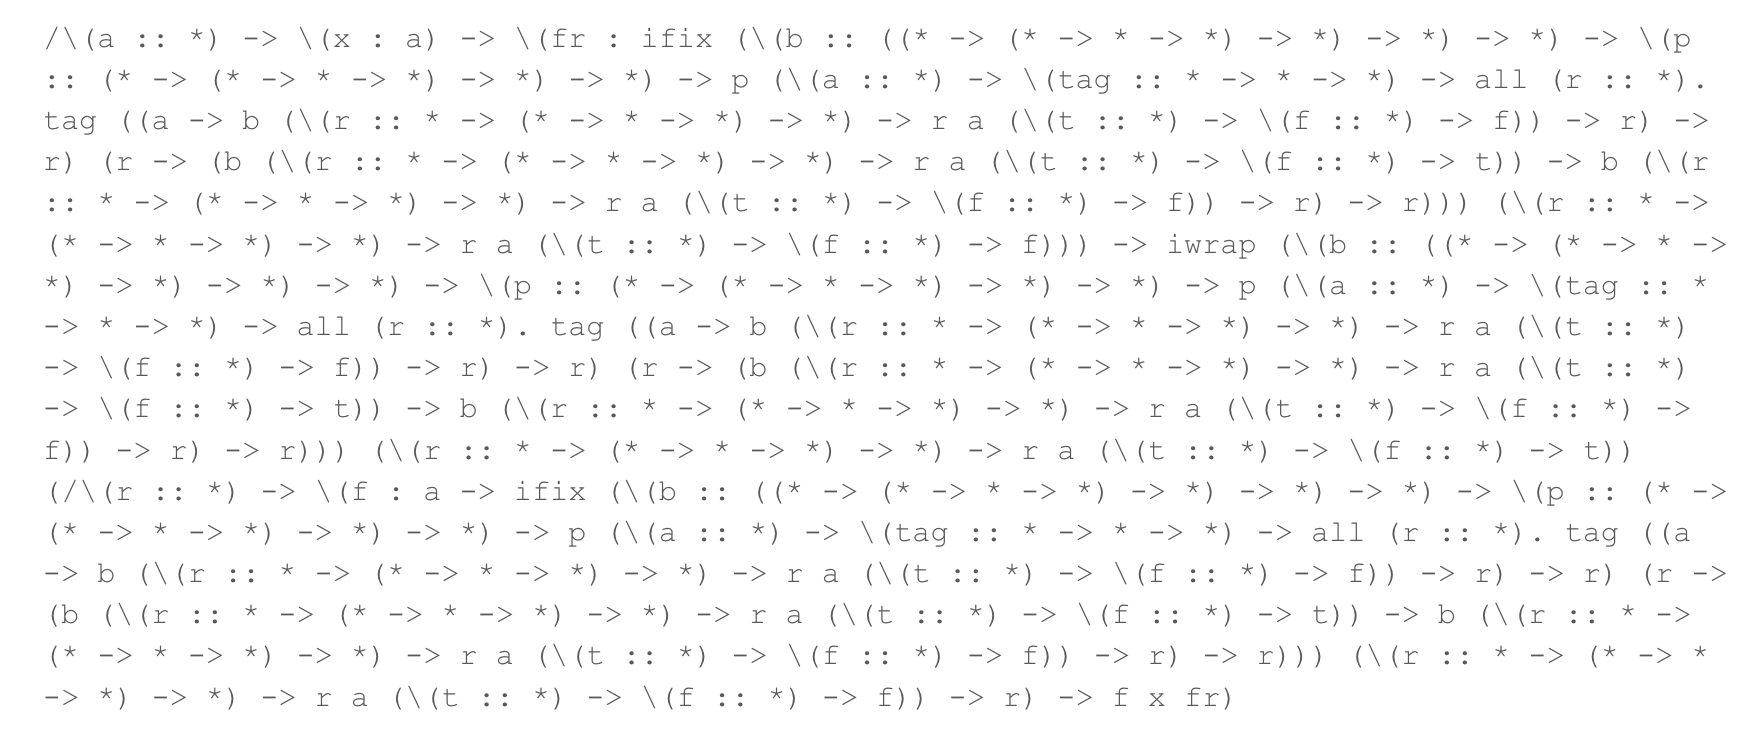
\includegraphics[scale=0.4]{images/node.png}

\end{columns}

\end{frame}

\section{Συνεισφορά}


\begin{frame}{Συνεισφορά}

\begin{itemize}[<+->]
    \item  Ορίσαμε μια πολύ \textbf{μικρή} και ταυτόχρονα \textbf{εκφραστική}
    γλώσσα
    \item Την μεταγλωττίσαμε σε γνωστά συστήματα του λ-λογισμού (\FOM + indexed fixpoints)
    \item
H \FIR{} υποστηρίζει και δήλωση αμοιβαία αναδρομικών όρων, γεγονός
που δεν έχει εξερευνηθεί στην βιβλιογραφία, σε γλώσσες με πρόθυμη αποτίμηση
    \item Οι προσπάθειες για κωδικοποίηση αμοιβαία αναδρομικών τύπων
    δεν εμπεριέχουν παραμετροποιημένους τύπους.
    \item
        Υλοποίηση (σε Agda) του compiler  είναι kind και type preserving.
    \item
        Υλοποίηση των παραπάνω σε πραγματικό σύστημα σε Haskell
\end{itemize}
\end{frame}

\begin{frame}{Συνεισφορά}

Τα αποτελέσματα της παραπάνω δουλειάς υποβλήθηκαν
στο συνέδριο συναρτησιακών γλωσσών ICFP19

\end{frame}

\begin{frame}{Μειονεκτήματα- Μελλοντικές κατευθύνσεις}

\begin{itemize}
    \item περισσότερη δουλειά στην θεωρία της \FIR{}
    \item semantics της \FIR{}, τα τωρινά semantics προκύπτων από
    την μεταγλώττιση σε \FOMF
    \item απόδειξη ότι η μεταγλώττιση είναι σωστή (αντιμετατίθεται
    με την αποτίμηση)
    \item εστιάζει στην ορθότητα και όχι στην απόδοση
\end{itemize}

\end{frame}

\begin{frame}{Σχετική βιβλιογραφία}

\begin{itemize}
\item<1->
Οι \citep*{BrownP17} εξετάζουν την \FOM με τους αναδρομικούς τύπους
που είδαμε, και παρόμοιο  \texttt{fixpoint} αλλά υποστηρίζουν μόνο
index με kind $\Type$

\item<2-> Στο \citep{scottenc} δίνεται περιγραφή της κωδικοποίησης Scott

\item<3->
Στο \citep{fixmutualgeneric} χρησιμοποιούν τον ίδιο fixpoint operator
και κωδικοποιούν τους αμοιβαία αναδρομικούς τύπους με χρήση τεχνικών
generic programming. δεν υποστηρίζουν παραμετροποιημένους τύπους.

\item<4->
Οι \citep*{henk} παρουσίασαν μια γλώσσα με ισχυρούς (dependent) τύπους
για χρήση ως ενδιάμεση αναπαράσταση σε συναρτησιακούς μεταγλωττιστές. Δεν
υποστηρίζουν ADTs και let-bindings

\end{itemize}

\end{frame}


\begin{frame}{Κώδικας}

Ο κώδικας της αρχιτεκτονικής plutus βρίσκεται εδώ:

  \begin{center}\url{github.com/input-output-hk/plutus/}\end{center}


\end{frame}

{\setbeamercolor{palette primary}{fg=black, bg=yellow}
\begin{frame}[standout]
  Ευχαριστώ!
\end{frame}
}

\appendix


\begin{frame}{Well-formedness}
  \begin{minipage}[t]{10cm}
    %\centering
    \begin{displaymath}
    \begin{array}{ll}
    \inference[W-Con]{c = x(\seq{T}) & \seq{\Gamma |- T::\Type}}{\Gamma \provesok c} \\
    \\
    \inference[W-Term]{
      \Gamma |- T :: \Type &
      \Gamma |- t : T}{\Gamma \provesok x : T = t} &
    \inference[W-Type]{\Gamma |- T :: K}{\Gamma \provesok X : K = T}\\
    \\
    \multicolumn{2}{l}{\inference[W-Data]{
      d=\datatype{X}{(\seq{Y :: K})}{x}{(\seq{c})} \\
      \Gamma^\prime = \Gamma, \seq{Y::K} &
      \seq{\Gamma^\prime \provesok c}}{\Gamma \provesok d}}\\
    \end{array}
    \end{displaymath}
    \end{minipage}

\end{frame}

\begin{frame}{Type Equivalence}
      \begin{minipage}[t]{10cm}
    \centering
    \begin{displaymath}
    \begin{array}{ll}
    \inference[Q-Refl]{}{T \equiv T} &
    \inference[Q-Symm]{T \equiv S}{S \equiv T}  \\
    \\
    \inference[Q-Trans]{S \equiv U & U \equiv T}{S \equiv T} &
    \inference[Q-Arrow]{S_1 \equiv S_2 & T_1 \equiv T_2}{(S_1 -> T_1) \equiv (S_2 -> T_2)} \\
    \\
    \inference[Q-All]{S \equiv T}{(\forall X::K.S) \equiv (\forall X::K.T)} &
    \inference[Q-Abs]{S \equiv T}{(\lambda X::K.S) \equiv (\lambda X::K.T)} \\
    \\
    \inference[Q-App]{S_1 \equiv S_2 & T_1 \equiv T_2}{S_1 T_1 \equiv S_2 T_2} &
    \inference[Q-Beta]{}{(\lambda X::K.T_1)T_2 \equiv \subst{X}{T_2}{T_1}}
    \end{array}
    \end{displaymath}
    \end{minipage}

 \end{frame}



 \begin{frame}{Κωδικοποίηση του Maybe}

\begin{align*}
\onslide<1->{
  &\compiledata(\tlet \datatype{\Maybe}{A}{\Match}{(\Nothing (), \Just (A))}\\
  &\quad\quad \tin\ \Match\ \{\Int\}\ (\Just \{\Int\}1)\ 0\ (\lambda x: \Int . x+1))\\
  =\ &(\Lambda (\Maybe :: \Type \kindArrow \Type) . \\}
  \onslide<2->{
  &\lambda (\Nothing : \forall A . \Maybe A) . \\}
  \onslide<3->{
  &\lambda (\Just : \forall A . A \rightarrow \Maybe A) . \\}
  \onslide<4->{
  &\lambda (\Match : \forall A . \Maybe A \rightarrow \forall R . R \rightarrow (A \rightarrow R) \rightarrow R). \\}
  \onslide<5->{
  &\Match\ \{\Int\}\ (\Just \{\Int\}1)\ 0\ (\lambda x: \Int . x+1)) \\}
  \onslide<6->{
  &(\lambda A . \forall R . R \rightarrow (A \rightarrow R) \rightarrow R) \\}
  \onslide<7->{
  &(\Lambda A . \Lambda R . \lambda (b_1 : R)\ (b_2 : A \rightarrow R) . b_1) \\}
  \onslide<8->{
  &(\Lambda A . \lambda (v_1 : A) . \Lambda R . \lambda (b_1 : R)\ (b_2 : A \rightarrow R) . b_2\ v_1) \\}
  \onslide<9->{
  &(\Lambda A . \lambda (v : \forall R . R \rightarrow (A \rightarrow R) \rightarrow R) . v) }
\end{align*}

\end{frame}


 \begin{frame}{Σύνθεση τύπων στην \FOMF}
 \begin{displaymath}
    \begin{array}{ll}
    \inference[K-TVar]{X::K \in \Gamma}{\Gamma |- X :: K} &
    \inference[K-Abs]{\Gamma, X::K_1 |- T :: K_2}{\Gamma |- (\lambda X::K_1.T) :: K_1 \kindArrow K_2} \\
    \\
    \inference[K-App]{\Gamma |- T_1 :: K_1 \kindArrow K_2 \\ \Gamma |- T_2 :: K_1}{\Gamma |- (T_1 ~ T_2) :: K_2} &
    \inference[K-Arrow]{\Gamma |- T_1 :: \Type & \Gamma |- T_2 :: \Type}{\Gamma |- (T_1 \rightarrow T_2) :: \Type} \\
    \\
    \inference[K-All]{\Gamma, X::K |- T :: \Type}{\Gamma |- (\forall X::K.T) :: \Type} &
    \fomfDiff{\inference[K-Ifix]{\Gamma |- T:: K \\ \Gamma |- F :: (K \kindArrow \Type) \kindArrow (K \kindArrow \Type)} {\Gamma |- (\ifix ~ F ~ T) :: \Type} }
    \end{array}
    \end{displaymath}

\end{frame}



\begin{frame}{Κωδικοποίηση Scott}

\begin{itemize}
    \item
Ο κλασσικός τρόπος κωδικοποίησης αλγεβρικών τύπων δεδομένων είναι η
κωδικοποίηση Church.

    \item Εμείς θα χρησιμοποιήσουμε την κωδικοποίηση Scott ,
    βελτίωση της Church που μας επιτρέπει να δουλέψουμε πιο αποδοτικά
    με αλγεβρικούς τύποιυς δεδομένων

\end{itemize}

\end{frame}



\begin{frame}{Τύποι δεδομένων}
  \begin{minipage}[t]{10cm}
      \centering
      \begin{displaymath}
      \begin{array}{l@{\ }l@{\ }l}
       \multicolumn{3}{l}{\textsf{Στις παρακάτω διαφάνειες έχουμε:}}\\
  \multicolumn{3}{l}{l = \tlet [\rec] \seq{d} \tin t} \\
  \multicolumn{3}{l}{d = \datatype{X}{(\seq{Y :: K})}{x}{(\seq{c})}} \\
  \multicolumn{3}{l}{c = x(\seq{T})}\\
  \\
  \multicolumn{3}{l}{\textsc{Auxiliary functions}}\\
  \constr{d}{c}
  &=& \Lambda (\seq{Y::K}) .
   \lambda (\seq{a : T}).
   \Lambda R .
   \lambda (\seq{b : \branchTy{c}{R}})
   ~b_i ~ \seq{a}\\
  &&\textbf{where}~c=c_i\\
  \constrs{d} &=& \seq{\constr{d}{c}}\\
  \match{d}
  &=& \Lambda (\seq{Y::K}). \lambda (x : (\scottTy{d}\ \seq{Y}) . x\\
  \unveil{d}{t}
  &=& \subst{X}{\scottTy{d}}{t} \\
  \\
  \multicolumn{3}{l}{\textsc{Compilation function}}\\
  \multicolumn{3}{l}{\compiledata(\tlet d \tin t)}\\
  &=& (\Lambda (\dataBind{d}) . \lambda (\constrBinds{d}) . \lambda (\matchBind{d}) . t)\\
  &&\{\scottTy{d}\}\ \\
  &&\seq{\unveil{d}{\constrs{d}}}\\
  &&\match{d}\\
    \end{array}
    \end{displaymath}
    \end{minipage}
\end{frame}

\begin{frame}{Κανόνες τύπων}

  \begin{minipage}[t]{10cm}
    \centering
    \begin{displaymath}
    \begin{array}{ll}

    \multicolumn{2}{l}{\inference[T-Let]{
    \Gamma \provesok \seq{b} &
    \Gamma |- T :: \Type &
    \Gamma, \seq{\binds{b}} |- t : T
    }
    { \Gamma |- (\tlet \seq{b} \tin t) : T
    }}\\
    \\
    \multicolumn{2}{l}{\inference[T-LetRec]{
    \Gamma, \seq{\binds{b}} \provesok \seq{b} &
    \Gamma |- T :: \Type &
    \Gamma, \seq{\binds{b}} |- t : T
    }
    { \Gamma |- (\tlet \rec \seq{b} \tin t) : T
    }}
    \end{array}
    \end{displaymath}
    \end{minipage}

\end{frame}


\begin{frame}[allowframebreaks]{References}
\bibliography{slides}

\end{frame}


\end{document}
